\label{indexX}
\ensurespace\section{Audacity Manual Contents}
\par\vspace{1mm}\hrule
\begin{multicols}{2}
\label{indexXtranslations}\textbf{Translation volunteers welcome...} If you'd like to help translate this Manual to other languages, please write to our feedback address for an account on this wiki.   
\par \protect
\includegraphics[max width=\linewidth]{C:/OpenSourceGit/AudacityTeamTools/test/m/images/8/8c/audacity_logo_whitebg.png}\par 
\subsection{Audacity 2.2.0 Manual}
\subsection{
\hyperref[\foo{manXnewXfeaturesXinXthisXreleaseX}]{New features in this release}
}\textbf{
\hyperref[\foo{manXfaqX}]{Frequently Asked Questions (FAQ)}
}\protect\includegraphics[max width=\linewidth]{C:/OpenSourceGit/AudacityTeamTools/test/m/images/b/b5/icon_faq.gif}  -  \textit{most common questions are answered in the FAQ}
\begin{itemize}
\item Search the Wiki for extra tips and tutorials
\item Visit the Forum for technical help
\item 
\hyperref[\foo{manXhowXtoXgetXhelpX}]{Using Help Resources}

\end{itemize}

\label{indexXreference}
\subsection{Guide to the Audacity Project Window}1\textbf{
\hyperref[\foo{manXmenuXreferenceX}]{Menu Bar}
}2\textbf{
\hyperref[\foo{manXtransportXtoolbarX}]{Transport Toolbar}
}3\textbf{
\hyperref[\foo{manXtoolsXtoolbarX}]{Tools Toolbar}
}4\textbf{
\hyperref[\foo{manXmeterXtoolbarXrecording}]{Recording Meter Toolbar}
}5\textbf{
\hyperref[\foo{manXmeterXtoolbarXplayback}]{Playback Meter Toolbar}
}6\textbf{
\hyperref[\foo{manXmixerXtoolbarX}]{Mixer Toolbar}
}7\textbf{
\hyperref[\foo{manXeditXtoolbarX}]{Edit Toolbar}
}8\textbf{
\hyperref[\foo{manXtranscriptionXtoolbarX}]{Transcription Toolbar}
}9\textbf{
\hyperref[\foo{manXdeviceXtoolbarX}]{Device Toolbar}
}10\textbf{
\hyperref[\foo{manXtimelineXpinned}]{Unpinned Play/Recording Head}
}11\textbf{
\hyperref[\foo{manXtimelineX}]{Timeline}
}12\textbf{
\hyperref[\foo{manXscrubbingXandXseekingXscrubbing}]{Scrub Ruler}
}13\textbf{
\hyperref[\foo{manXtrackXcontrolXpanelXandXverticalXscaleX}]{Track Control Panel}
}14\textbf{
\hyperref[\foo{manXaudioXtracksX}]{Audio Track}
}15\textbf{
\hyperref[\foo{manXlabelXtracksX}]{Label Track}
}16\textbf{
\hyperref[\foo{manXselectionXtoolbarX}]{Selection Toolbar}
}17\textbf{
\hyperref[\foo{manXstatusXbarX}]{Status Bar}
}\textbf{Hover over and click on the image to learn more.}
\hyperref[\foo{indexXXskiptheimage}]{Skip the image}
\par \protect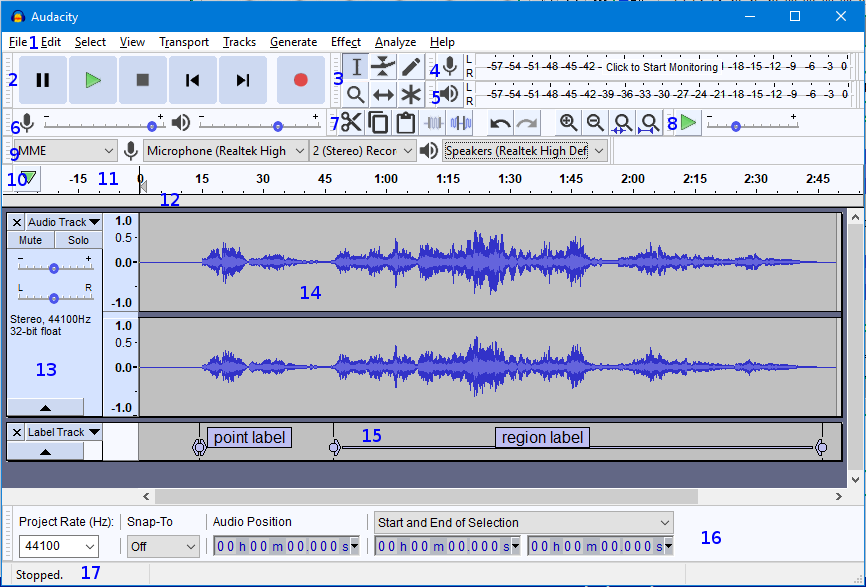
\includegraphics[max width=\linewidth]{C:/OpenSourceGit/AudacityTeamTools/test/m/images/7/7a/projectwindowimagemap_220.png}\par 
\paragraph{Help buttons}
\begin{itemize}
\item \protect
\includegraphics[max width=\linewidth]{C:/OpenSourceGit/AudacityTeamTools/test/m/images/d/d6/help_button.png} Some places in Audacity have a help button, click for the relevant Manual page.
\end{itemize}

\paragraph{Additional Menus on Mac}
\begin{itemize}
\item 
\hyperref[\foo{manXaudacityXmenuX}]{Audacity}

\item 
\hyperref[\foo{manXwindowXmenuX}]{Window}

\end{itemize}

\label{indexXrefXbottom}
\label{indexXskiptheimage}
\label{indexXtutorials}
\subsection{Tutorials}
\begin{itemize}
\item 
\hyperref[\foo{manXtutorialXeditingXanXexistingXfileX}]{Editing an Audio File}
 - Import the file, edit and export it
\item 
\hyperref[\foo{manXtutorialXyourXfirstXrecordingX}]{Your First Recording}
 - Record microphone, guitar, keyboard
\item 
\hyperref[\foo{manXtutorialXmixingXaXnarrationXwithXbackgroundXmusicX}]{Mixing Voice with Background Music}
 - For podcasts
\item 
\hyperref[\foo{manXtutorialXrecordingXmultiXtrackXoverdubsX}]{Recording Multi-track Overdubs}
 - Record over other tracks
\item 
\hyperref[\foo{manXtutorialXvocalXremovalXandXisolationX}]{Vocal Removal and Isolation}

\item 
\hyperref[\foo{manXtutorialXloopingX}]{Looping}
 - make an audio loop with Audacity
\item 
\hyperref[\foo{manXtutorialXmakingXringtonesXandXivrXmessagesX}]{Making Ringtones and IVR messages}
 - For your cellphone or IVR system
\item 
\hyperref[\foo{manXtutorialXrecordingXaudioXplayingXonXtheXcomputerX}]{Recording streaming audio playing on the computer}

\end{itemize}

\begin{itemize}
\item 
\hyperref[\foo{manXtutorialXcopyingXtapesXlpsXorXminidiscsXtoXcdX}]{Copying tapes, LPs and other media to CD or computer}

\item 
\hyperref[\foo{manXtutorialXclickXandXpopXremovalXtechniquesX}]{Click and pop removal techniques}

\item 
\hyperref[\foo{manXsplittingXaXrecordingXintoXseparateXtracksX}]{Splitting a recording into separate tracks}

\item 
\hyperref[\foo{manXburningXmusicXfilesXtoXaXcdX}]{Burning Audio CDs}
 and 
\hyperref[\foo{manXtutorialXhowXtoXimportXcdsX}]{How to import CDs}

\item 
\hyperref[\foo{manXsampleXworkflowXforXlpXdigitizationX}]{Sample workflow for LP digitization}
 and 
\hyperref[\foo{manXsampleXworkflowXforXtapeXdigitizationX}]{Sample workflow for tape digitization}

\end{itemize}

\begin{itemize}
\item 
\hyperref[\foo{manXtutorialXexportingXtoXitunesX}]{Exporting to iTunes}
 and 
\hyperref[\foo{manXtutorialXhowXtoXimportXfilesXfromXitunesX}]{Importing from iTunes}

\item 
\hyperref[\foo{manXsampleXworkflowXforXexportingXtoXitunesX}]{Sample workflow for exporting to iTunes}

\end{itemize}

\begin{itemize}
\item 
\hyperref[\foo{manXrecordingX78XrpmXrecordsX}]{Recording 78 rpm records}

\end{itemize}

\label{indexXbottomXusing}
\label{indexXusing}
\subsection{Using Audacity}
\subsubsection{Quick Help}
\begin{itemize}
\item 
\hyperref[\foo{quickXhelpX}]{Getting Started}
 - Recording, Importing, Editing, Exporting...

\begin{itemize}
\item 
\hyperref[\foo{manXaudacityXtourXguideX}]{Audacity Tour Guide}
 - quick tour of selected features of Audacity
\end{itemize}

\item Installing and updating Audacity on 
\hyperref[\foo{manXinstallingXandXupdatingXaudacityXonXwindowsX}]{Windows}
, 
\hyperref[\foo{manXinstallingXandXupdatingXaudacityXonXmacXosXxX}]{Mac}
 or 
\hyperref[\foo{manXinstallingXandXupdatingXaudacityXonXlinuxX}]{Linux}

\item Installing plug-ins for Audacity on 
\hyperref[\foo{manXinstallingXeffectXgeneratorXandXanalyzerXplugXinsXonXwindowsX}]{Windows}
, 
\hyperref[\foo{manXinstallingXeffectXgeneratorXandXanalyzerXplugXinsXonXmacXosXxX}]{Mac}
 or 
\hyperref[\foo{manXinstallingXeffectXgeneratorXandXanalyzerXplugXinsXonXlinuxX}]{Linux}

\item 
\hyperref[\foo{manXthemesX}]{Themes}
 - learn how to select your preferred Audacity look and feel
\end{itemize}

\subsubsection{Audacity Foundations}
\begin{itemize}
\item 
\hyperref[\foo{manXaudacityXprojectsX}]{Managing Audacity Projects}
 - Audacity's internal workspace 
\item 
\hyperref[\foo{manXaudacityXsetupXandXconfigurationX}]{Audacity Setup and Configuration}

\begin{itemize}
\item 
\hyperref[\foo{manXpreferencesX}]{Preferences}
 - changing your settings and 
\hyperref[\foo{manXfaqXinstallationXandXplugXinsXreset}]{reset to default}

\end{itemize}

\item 
\hyperref[\foo{manXtoolbarsXoverviewX}]{Toolbars Overview}
 - including how to arrange Toolbars
\item 
\hyperref[\foo{manXaudioXtracksX}]{Audio Tracks}
, 
\hyperref[\foo{manXaudacityXwaveformX}]{Waveform view}
 and 
\hyperref[\foo{manXspectrogramXviewX}]{Spectrogram view}

\begin{itemize}
\item 
\hyperref[\foo{manXtrackXcontrolXpanelXandXverticalXscaleX}]{Track Control Panel and Vertical Scale}

\item 
\hyperref[\foo{manXlabelXtracksX}]{Label Tracks}

\item 
\hyperref[\foo{manXtimeXtracksX}]{Time Tracks}

\item 
\hyperref[\foo{manXnoteXtracksX}]{Note Tracks}

\end{itemize}

\item 
\hyperref[\foo{manXplayingXandXrecordingX}]{Playing and Recording}
, 
\hyperref[\foo{manXtimelineXtqp}]{Quick-Play}
, 
\hyperref[\foo{manXscrubbingXandXseekingX}]{Scrubbing}
 and 
\hyperref[\foo{manXtimerXrecordX}]{Timer Recording}

\item 
\hyperref[\foo{manXimportingXaudioX}]{Importing audio}
 and 
\hyperref[\foo{manXexportingXaudioX}]{Exporting audio files}
 - For use in other applications

\begin{itemize}
\item 
\hyperref[\foo{manXfaqXinstallationXandXplugXinsXlame}]{LAME MP3 export}
 and 
\hyperref[\foo{manXfaqXinstallationXandXplugXinsXffdown}]{FFmpeg import/export}
 libraries for more formats
\item 
\hyperref[\foo{manXonXdemandXloadingX}]{On-Demand Loading}
 of uncompressed files
\item 
\hyperref[\foo{manXmetadataXeditorX}]{Metadata Editor}

\end{itemize}

\item 
\hyperref[\foo{manXnavigationXtipsX}]{Navigation Tips}
, 
\hyperref[\foo{manXplaybackXtipsX}]{Playback Tips}
 and 
\hyperref[\foo{manXaudioXalignmentXtipsX}]{Audio Alignment Tips}

\item 
\hyperref[\foo{manXkeyboardXshortcutXreferenceX}]{Keyboard shortcuts}

\end{itemize}

\subsubsection{Editing with Audacity}
\begin{itemize}
\item 
\hyperref[\foo{manXaudacityXselectionX}]{Selecting audio}
 and 
\hyperref[\foo{manXspectralXselectionX}]{Spectral Selection}

\item 
\hyperref[\foo{manXaudacityXtracksXandXclipsX}]{Clips - individual sections within an Audio Track}

\item 
\hyperref[\foo{manXsplittingXandXjoiningXstereoXtracksX}]{Splitting and Joining Stereo Tracks}

\item 
\hyperref[\foo{manXzoomingX}]{Zooming Overview}

\item 
\hyperref[\foo{manXindexXofXeffectsXgeneratorsXandXanalyzersX}]{Effects}
, 
\hyperref[\foo{manXindexXofXeffectsXgeneratorsXandXanalyzersXgenerators}]{Generators}
 and 
\hyperref[\foo{manXindexXofXeffectsXgeneratorsXandXanalyzersXanalyzers}]{Analyzers}

\item 
\hyperref[\foo{manXcreatingXaXcrossfadeX}]{Creating a Crossfade}

\item 
\hyperref[\foo{manXmixingX}]{Mixing Audio Tracks}

\item 
\hyperref[\foo{manXundoXredoXandXhistoryX}]{Undo, Redo and History}

\end{itemize}

\subsubsection{Help with Advanced Topics}
\begin{itemize}
\item 
\hyperref[\foo{manXaccessibilityX}]{Accessibility}
 - Audacity for the visually impaired 
\item 
\hyperref[\foo{manXlatencyXtestX}]{Latency when recording overdubs}

\item 
\hyperref[\foo{manXcustomizationX}]{Adding plug-ins \& other customization}
, 
\hyperref[\foo{manXscriptingX}]{Scripting}
 and 
\hyperref[\foo{manXsimplifyingXaudacityX}]{Simplifying Menus}

\item 
\hyperref[\foo{manXchainsXforXbatchXprocessingXandXeffectsXautomationX}]{Chains - for batch processing and effects automation}

\item 
\hyperref[\foo{manXsyncXlockedXtrackXgroupsX}]{Sync-Locked Track Groups}

\item 
\hyperref[\foo{manXtimeXtracksX}]{Time Tracks}
 - used for varying speed control
\item 
\hyperref[\foo{manXrecoveryX}]{Crash Recovery}

\end{itemize}

\label{indexXbottomXusing}
\label{indexXmisc}
\subsection{Index, Glossary and More}
\begin{itemize}
\item 
\hyperref[\foo{manXsubjectXindexX}]{Subject Index}

\item 
\hyperref[\foo{manXglossaryX}]{Glossary of Terms}

\item 
\hyperref[\foo{manXcreditsX}]{Credits}

\end{itemize}

\begin{itemize}
\item 
\hyperref[\foo{manXlicenseX}]{Audacity License}

\item 
\hyperref[\foo{manXinformationXforXdevelopersX}]{Information for Developers}
 - join our developer community
\end{itemize}

\label{indexXmiscXbottom}\vspace{1mm}\hrule \textbf{Links:} Most links are to other pages in this Manual. \textit{\textbf{Bold italicized}}  links are to a description in our 
\hyperref[\foo{manXglossaryX}]{Glossary}
. Other \textit{italicised}  links are to pages external to this Manual, mostly to our main website or Wiki. We are not responsible for the content of any other external sites.    
\textbf{Screenshots:} Unless otherwise stated, screenshots in this Manual are of Audacity running 
under its 
\hyperref[\foo{manXpreferencesXstored}]{default settings}
 on the Microsoft Windows 10® operating system. Representative images of Audacity running on Mac and Linux are also included. 
\textbf{Copyright:} Unless otherwise noted, all pages in this Manual are available under the terms of the Creative Commons Attribution 3.0 license. In essence, you are free to (1) copy, distribute and transmit the work (2) to adapt the work, under condition you must \textbf{attribute} the work to the authors (but not in any way that suggests that they endorse you or your use of the work). For any reuse or distribution, you must make clear to others the license terms of this work. Any of the above conditions can be waived if you get permission from us.
\end{multicols}